According to \citeauthor{Keim2010}, visual analytics "[\ldots] is not easy to define, due to its multi-disciplinary nature involving multiple processes and the wide variety of application areas \iacite{Keim2010}." Based on current practice, they define visual analytics as the combination of automated analysis techniques with interactive visualisations for an effective understanding, reasoning and decision-making on the basis of very large and complex datasets \iacite{Keim2010}.

So, based on the definition, \citeauthor{Keim2010} elaborate the objectives of visual analytics to state that it is the creation of tools and techniques to enable people to:

\begin{itemize}
\item Summarize information and derive insight from heterogeneous and often conflicting data
\item Detect the expected and discover the unexpected
\item Provide reasonable and understandable evaluations
\item Communicate these evaluations effectively for action
\end{itemize}

The following part of this chapter gives an overview of how visual analytics tries to achieve these objectives to generate knowledge from data. Based upon the knowledge gathered in this chapter and the chapters before, it is possible to derive design principles for good visualisations.

Figure \ref{fig:va-process} on page \pageref{fig:va-process} shows an abstract overview of the visual analytics process. It contains different stages, represented as colored ovals, and their corresponding transitions, represented as arrows. The first step of the process deals with the integration of heterogeneous data sources. This integration includes tasks like data preprocessing, transforming, cleaning, normalization, grouping, and fusion. All those tasks are indicated by the transformation transition onto the data oval. After the transformation, the analyst has two different options to choose \iacite{Keim2010}:

\begin{enumerate}
\ditem{Automated data analysis} \hfill \\
If an automated model was chosen first, data mining methods are applied to generate statistical models out of the original data. Once the model is made, the analyst only needs to refine its parameters and evaluate it afterwards. The advantage of this choice is the scalability because it can be fully automatized. This automatization is also the main disadvantage. The model runs in a black box fashion, ignoring all interactions. If this is done, the evaluation of the model can be accomplished with a visualisation. This makes it possible to interact with the data later on \iacite{Keim2010}.

\ditem{Visual data exploration} \hfill \\
If visual data exploration is chosen first, interaction with the generated visualisation is needed to construct insightful information. Interaction could be integrated by zooming or considering different views on the data. Findings can be used to create automatic models. The main advantage of this approach is the interaction with an analyst, thus offering more flexibility and possibilities. On the other hand, it is not scaleable in any way.
\end{enumerate}

\begin{figure}[!htb]
\centering
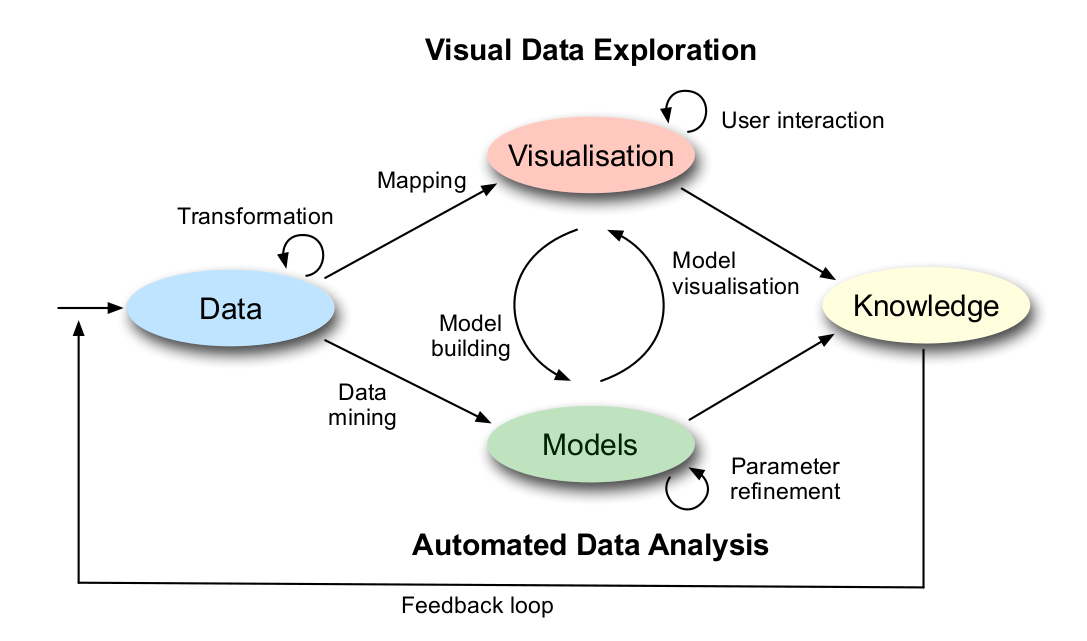
\includegraphics[height=5cm,keepaspectratio]{images/va/va-process.png}
\caption[
    The visual analytics process is characterised through interaction between data, visualisations, models about the data and the users in order to discover knowledge \iacite{Keim2010}.
]{The visual analytics process is characterised through interaction between data, visualisations, models about the data and the users in order to discover knowledge.}
\label{fig:va-process}
\end{figure}

If automated data and visual data analysis are used in an agile way like iterating both analysis methods in sequence until knowledge is discovered, misleading results in an intermediate step can be discovered and eliminated at an early stage and thus leading to higher confidence and better results \iacite{Keim2010}.

In summary, it can be said that the visual analytics process extracts knowledge gained from visualisations, automatized analysis, and a human analyst combining these two.

Figure \ref{fig:va-related} on page \pageref{fig:va-related} shows the interdisciplinary character of visual analytics. With visualisation as its core, other disciplines like data management, data analysis, and data mining are close related and seem kind of obvious based on the knowledge of the visual analytics process and the definition of the term itself.

\begin{figure}[!htb]
\centering
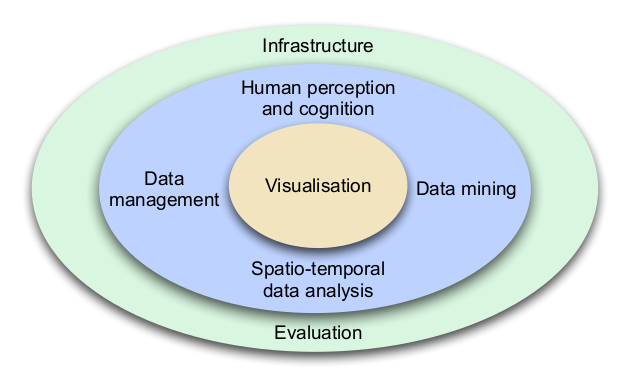
\includegraphics[height=5cm,keepaspectratio]{images/va/va-related.png}
\caption[
    Visual analytics with core adjacent disciplines \iacite{Keim2010}.
]{Visual analytics with core adjacent disciplines.}
\label{fig:va-related}
\end{figure}

In order to create visualisation designs, it is needed to clarify the usage of marks and channels in designs first. Marks basically are geometric elements that depict items or links. Figure \ref{fig:va-marks} on page \pageref{fig:va-marks} shows examples of marks in different dimensions. Points count as a 0D mark, whereas lines belong to 1D marks, and areas to 2D marks. A visual channel controls the appearance of a given mark, independent of the dimensionality. Figure \ref{fig:va-channels} on page \pageref{fig:va-channels} shows a few channels that can encode information. The core of a design can be described as a combination of two aspects: graphical elements called marks, and visual channels.

\begin{figure}[!htb]
\centering
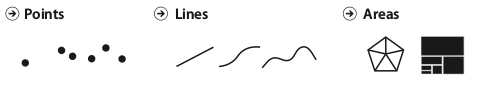
\includegraphics[width=0.5\textwidth,keepaspectratio]{images/va/marks.png}
\caption[
    Marks are geometric primitives \iacite{Munzner2014}.
]{Marks are geometric primitives.}
\label{fig:va-marks}
\end{figure}

\citeauthor{Munzner2014} states that all channels are not equal. She says using two different visual channels on the same data attribute results in different information after it has passed through the perceptual and cognitive processes of the human visual system. The usage of marks and channels in a design should be guided by the principles of expressiveness and effectiveness \iacite{Munzner2014}.

\begin{figure}[!htb]
\centering
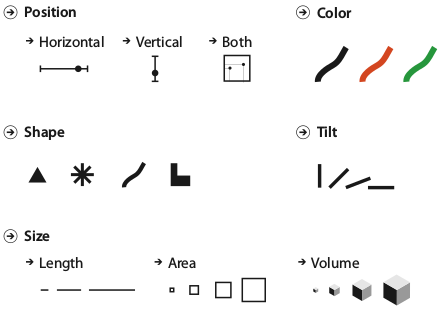
\includegraphics[height=5cm,keepaspectratio]{images/va/channels.png}
\caption[
    Visual channels control the appearance of marks \iacite{Munzner2014}.
]{Visual channels control the appearance of marks.}
\label{fig:va-channels}
\end{figure}

\begin{enumerate}
\ditem{The expressiveness principle} suggests that the used channel should express all of the information in the dataset attributes. The most fundamental expression of this principle is, that known pattern should be shown accordingly, e.g. sorted and ranked data should be shown in a way that this pattern is intrinsically sensed \iacite{Munzner2014}.

\ditem{The effectiveness principle} suggests that the importance of the data attribute should match the emphasis of the channel, so to say its noticeability \iacite{Munzner2014}.
\end{enumerate}

Figure \ref{fig:va-channels-ranked} on page \pageref{fig:va-channels-ranked} introduces visual channels ranked by their effectiveness. To fully understand this figure, it is first needed to explain different attribute types.

There are two major types: categorical and ordered. Within the ordered type, there is a distinction between ordinal and quantitative types. Categorical data attributes can be mathematically described as the attributes where only equality comparisons of attributes are possible ($=$, $\neq$). This does not exclude the usage of any arbitrary external ordering like alphabetically ordering because such orderings are not implicit in the attribute itself. However, ordered data allows the use of ranking in addition to equality comparisons because they have such an implication ($=$, $\neq$, $>$, $<$). As already mentioned, this type can be further subclassified. Quantitative data allow the usage of arithmetic operations because it is a measurement of magnitude. Only one further distinction is needed to know if multiplication and division are possible or not. If the origin of the measurement is meaningful, like in length, mass, temperature, and so forth, it is possible to use the following arithmetic operations: $=$, $\neq$, $>$, $<$, $+$, $-$, $\times$, $\div$. If this is not the case, but the attribute still allows for zero arbitrary, the following arithmetic operations can be applied: $=$, $\neq$, $>$, $<$, $+$, $-$ \iacite{Stevens1946}.

\begin{figure}[!htb]
\centering
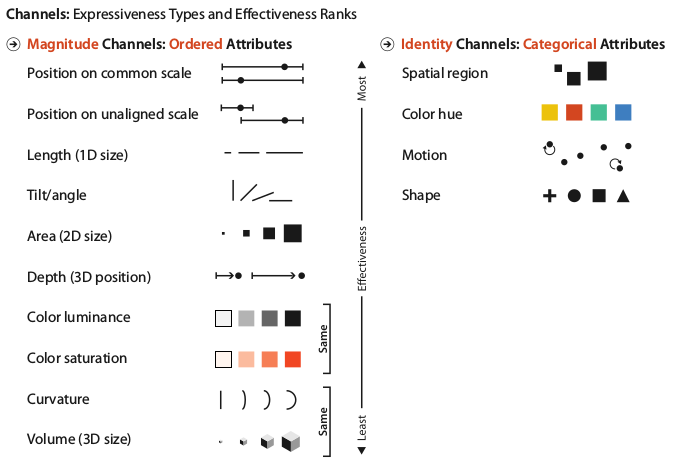
\includegraphics[height=10cm,keepaspectratio]{images/va/channels-ranked.png}
\caption[
    Channels ranked by effectiveness according to data and channel type. Ordered data should be shown with the magnitude channels, and categorical data with the identity channels \iacite{Munzner2014}.
]{Channels ranked by effectiveness according to data and channel type. Ordered data should be shown with the magnitude channels, and categorical data with the identity channels.}
\label{fig:va-channels-ranked}
\end{figure}

With the different attribute types defined and explained, the distinction and usage of magnitude and identity channels, visible in figure \ref{fig:va-channels-ranked}, should be clear. The ranking ranges from the most effective channels at the top to the least effective ones at the bottom. The most effective visual channels for ordered attributes are based on spatial position, either aligned or unaligned. The next four channels (length, angle, area and depth) are somewhat combinable: length is a 1D size, whereas angle and area are used for 2D sizes and depth for 3D positioning. These channels are followed by two roughly equally effective ones: luminance and saturation, which in turn are followed by two channels roughly equal in terms of effectiveness: curvature and volume. The most effective identity channel is spatial region, followed by color hue. In third position is the motion channel, which is very effective for a single set of moving items against a sea of static ones. The least effective channel is the shape \iacite{Munzner2014}.

It is observable, that both channels have 2D spatial positioning ranked highest. The ranking shown is \citeauthor{Munzner2014}'s own synthesis of information drawn from many sources. The justification of this ranking is not part of this thesis and will be not be discussed.